\newpage
\chapter{Fluxo de Gradiente em Espaços de Wasserstein}

Neste capítulo mostraremos como EDPs podem ser expressadas como
Fluxos de Gradiente em um espaço de Wasserstein
(i.e. espaço métrico de medidas de probabilidades com distância de Wasserstein). A exposição é
focada em apresentar de maneira clara e sucinta o necessário para entendimento
do assunto, sem provar os resultados mais refinados, o que tornaria o
texto muito extenso e de difícil entendimento\footnote{Fluxo de Gradientes é uma área por si só, assim, sugerimos ao leitor nesta área
que consulte \citet{ambrosio2008gradient}}.

Seja uma função $F:\mathbb R^n \to \mathbb R \in C^1$, e $x_0 \in \mathbb R^n$,
onde queremos descobrir $x(t)$ que resolve o seguinte sistema de equações:
\begin{equation}
    \begin{cases}
        x'(t) = -\nabla F(x(t)), \ t>0,\\
        x(0)  = x_0.
    \end{cases}
\end{equation}
A solução $x(t)$ do sistema acima será uma curva iniciando em $x_0$ e se movendo
na direção de menor gradiente, ou seja, a solução é dada
pelo famoso algoritmo de descida de gradiente. Em outras palavras,
a solução $x(t)$ caracteriza um Fluxo de Gradiente\footnote{Essa definição é informal. O conceito
de Fluxo de Gradiente será formalizado na seção seguinte.}.

Esse problema é simples quando estamos em espaços de dimensão finita e com
funções diferenciáveis, porém, torna-se mais
interessante e complexo quando começamos a considerar espaços de dimensão infinita
como $\mathcal P_2(\mathbb R^n)$. Neste cenário, temos que repensar, por exemplo,
a ideia de gradiente, já que não está mais claro que seria o gradiente quando
$x(t) = \rho_t \in \mathcal P_2(\mathbb R^n)$. Além disso, $F$ não é mais uma
função de $\mathbb R^n$ em $\mathbb R$, mas um funcional atuando em medidas
de probabilidade.

É interessante observar que, uma vez que consigamos reformular EDPs
como Fluxos de Gradiente em Wasserstein, poderemos utilizar resultados
obtidos nessa área para provar, por exemplo, existência e unicidade.

\section{Introdução aos Fluxos de Gradiente}

Antes de formalizar a ideia de fluxo de gradiente, vamos introduzir algumas
noções de análise convexa e cálculo das variações que são necessárias para tratar
do assunto de maneira rigorosa.

\begin{definition}[Subdiferencial]
    Seja $f:\mathbb R^n \to (-\infty, +\infty]$ própria, ou seja, $f(x) \neq +\infty \forall x$.
    O subdiferencial de $f$ é dado por:
    \begin{equation}
        \partial f(x) := \{p \in \mathbb R^n:
        f(y) \geq f(x) + \langle p, y-x\rangle, \forall y \in \mathbb R^n
        \}.
    \end{equation}
\end{definition}
A intuição por trás da definição
de subdiferencial (ou subgradiente) é ilustrada na Figura \ref{fig:subdiferencial}.
Note que se a função $f$ for convexa e diferenciável, teremos que $\partial f(x) = \{\nabla f(x)\}$.
Porém, caso a função não seja convexa, não haverá essa garantia. Assim, é comum usar essa ideia de
subdiferencial somente em funções convexas. A generalização dessa ideia de subdiferencial é dada
pela seguinte definição.

\begin{definition}[Subdiferencial Generalizado]
    \footnote{\citet{ambrosio2021lectures} chama de Gateaux subdifferencial.}
    Seja $f:\mathbb R^n \to (-\infty, +\infty]$ própria, ou seja, $f(x) \neq +\infty \forall x$.
    O subdiferencial generalizado de $f$ é dado por:
    \begin{equation}
        \partial_G g(x):= \{p \in \mathbb R^n: \liminf_{t\to 0^+}\frac{f(x+tv) - f(x)}{t}
        \geq \langle p,v \rangle v \in \mathbb R^n\}.
    \end{equation}
    Onde $t \to 0^+$ simboliza que $t$ tendo a $0$ pela direita.
\end{definition}

\begin{figure}[H]
    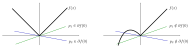
\includegraphics[width=1\textwidth]{./Figures/subdiferencial}
    \caption{Exemplo de subdiferencial.}
    \label{fig:subdiferencial}
\end{figure}
